
\section{Objective and Approach}\label{sec:objective_approach}

Our central aim is to understand the extent to which job postings convey meaningful information about the 
actual requirements of a position, specifically regarding skill fit. We investigate this by analyzing 
patterns in internal hiring decisions, under the premise that these decisions implicitly reveal the skills and 
demands prioritized by the organization.

Job postings utilize varied language to describe complex technical skills. Similar underlying requirements might 
be expressed differently across postings, while seemingly disparate descriptions could indicate similar skill needs. 
Internal mobility offers a valuable context for studying posting informativeness, as we observe both the textual 
content of position descriptions and the outcomes of employee transitions between roles. If postings effectively 
communicate skill requirements, we expect differences in their content to correlate with these transitions.

To formalize our investigation, consider an internal applicant being evaluated for a new role. Let $j_c$ denote 
the text of the applicant's current job posting and $j_v$ the text of the vacancy posting. The hiring manager 
considers various factors, some unobserved by us, represented by the feature vector $z_i$. We can model the 
selection decision as dependent on a distance measure $\delta(j_v, (j_c, z_i))$ between the vacancy and the 
applicant's profile, with selection occurring if this distance is below a threshold $\tau$:

\[
S(j_v, (j_c, z_i)) = 
\begin{cases} 
1, & \text{if } \delta(j_v, (j_c, z_i)) < \tau \\
0, & \text{if } \delta(j_v, (j_c, z_i)) \geq \tau
\end{cases}
\]


Given that we do not observe the full set of features $z_i$ considered in the actual selection process, our ability 
to perfectly predict individual hiring decisions based solely on job posting content is limited. We use the 
Area Under the Receiver Operating Characteristic Curve (AUC) to assess the extent to which the distance between 
job postings, derived from their text, aligns with observed hiring outcomes, recognizing that this metric 
provides a measure of how informative the postings are in accounting for skill fit, even with the presence 
of unobserved factors.

Our approach is guided by two key principles in representing and comparing job postings. First, we leverage 
the sophisticated language understanding capabilities of pre-trained transformer models to generate numerical 
representations (embeddings) of the posting text. The ability of these models to capture nuanced semantic 
relationships within large text corpora makes them well-suited for representing the specialized vocabulary 
of IT job descriptions, and their pre-trained nature offers significant practical advantages. Second, we 
utilize our historical selection decisions in a supervised manner to learn a distance metric between these embeddings. 
This process of metric learning allows us to fine-tune the distance measure, weighting differences in the 
embeddings according to their relevance in predicting observed hiring outcomes. This supervision allows us to 
extract signals related to the organization's implicit valuation of skills, as revealed through its hiring choices.


A critical aspect of our methodology is addressing the challenges associated with the high dimensionality of embeddings 
generated by large language models. One key motivation for dimensionality reduction is that learning a meaningful distance 
metric, which involves assigning appropriate weights to different dimensions, becomes increasingly difficult in 
high-dimensional spaces, particularly with a limited number of observed selection decisions. Furthermore, the 
embeddings of job postings, even for distinct roles within a single organization, are anticipated to exhibit a 
tendency to cluster within the broader embedding space. Therefore, we employ dimensionality reduction techniques 
to map these high-dimensional representations to a lower-dimensional space, aiming to distill the most salient 
features relevant to distinguishing between job requirements and facilitating effective metric learning.


\begin{figure}[t]
    % Add the necessary TikZ libraries if not already in preamble
    \usetikzlibrary{shapes.geometric, shapes.symbols, arrows, positioning, calc, matrix}
    
    \centering
    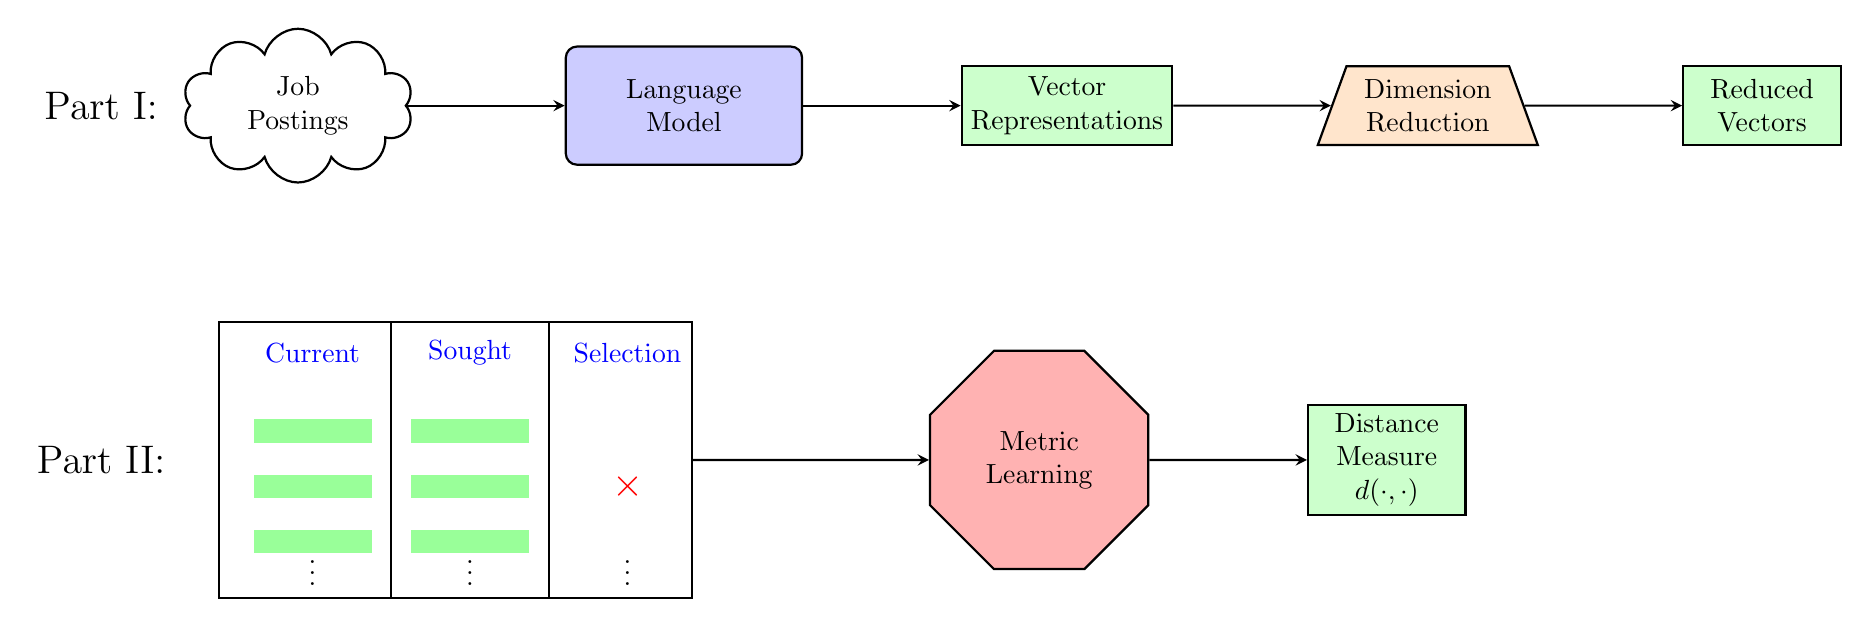
\begin{tikzpicture}[
        >=stealth,
        % Part I styles
        textinput/.style={cloud, draw, thick, aspect=2, minimum width=2cm, align=center},
        lmodel/.style={rectangle, draw, thick, rounded corners, fill=blue!20, minimum width=3cm, minimum height=1.5cm, align=center},
        vector/.style={rectangle, draw, thick, minimum width=2cm, minimum height=1cm, fill=green!20, align=center},
        reduction/.style={trapezium, trapezium angle=70, draw, thick, minimum width=2cm, minimum height=1cm, fill=orange!20, align=center},
        % Part II styles
        datainput/.style={rectangle, draw, thick, minimum width=6cm, minimum height=3.5cm},
        learning/.style={regular polygon, regular polygon sides=8, draw, thick, minimum size=3cm, fill=red!30, align=center},
        vectorbar/.style={rectangle, draw=none, fill=green!40, minimum width=1.5cm, minimum height=0.3cm},
        arrow/.style={thick, ->}
    ]
        % [Rest of the TikZ code exactly as in your working version]
        % Part I Label
        \node[align=left] at (-2.5,0) {\Large Part I:};
        
        % Part I Components
        \node (jobs) [textinput] at (0,0) {Job\\Postings};
        \node (llm) [lmodel, right=2cm of jobs] {Language\\Model};
        \node (vec_rep) [vector, right=2cm of llm] {Vector\\Representations};
        \node (reduce) [reduction, right=2cm of vec_rep] {Dimension\\Reduction};
        \node (red_vec) [vector, right=2cm of reduce] {Reduced\\Vectors};
        
        % Part I Connections
        \draw[arrow] (jobs) -- (llm);
        \draw[arrow] (llm) -- (vec_rep);
        \draw[arrow] (vec_rep) -- (reduce);
        \draw[arrow] (reduce) -- (red_vec);
        % Part II Label
        \node[align=left] at (-2.5,-4.5) {\Large Part II:};
        
        % Part II Components
        % Data input block
        \node (data) [datainput] at (2,-4.5) {};
        
        % Column headers
        \node[text=blue] at ($(data.north west)+(1.2,-0.4)$) {Current};
        \node[text=blue] at ($(data.north west)+(3.2,-0.4)$) {Sought};
        \node[text=blue] at ($(data.north west)+(5.2,-0.4)$) {Selection};
        
        % Vertical separators
        \draw[thick] ($(data.north west)+(2.2,0)$) -- ($(data.south west)+(2.2,0)$);
        \draw[thick] ($(data.north west)+(4.2,0)$) -- ($(data.south west)+(4.2,0)$);
        
        % Sample data rows with vector bars and check/cross
        \foreach \i [count=\yi] in {1,...,3}{
            \node[vectorbar] at ($(data.north west)+(1.2,-0.7-\yi*0.7)$) {};
            \node[vectorbar] at ($(data.north west)+(3.2,-0.7-\yi*0.7)$) {};
        }
        
        % Selection symbols
        \node[text=green!50!black] at ($(data.north west)+(5.2,-1.4)$) {\Large $\checkmark$};
        \node[text=red] at ($(data.north west)+(5.2,-2.1)$) {\Large $\times$};
        \node[text=green!50!black] at ($(data.north west)+(5.2,-2.8)$) {\Large $\checkmark$};
        
        % Dots for continuation
        \node at ($(data.north west)+(1.2,-3.1)$) {$\vdots$};
        \node at ($(data.north west)+(3.2,-3.1)$) {$\vdots$};
        \node at ($(data.north west)+(5.2,-3.1)$) {$\vdots$};
        
        % Metric learning and output
        \node (metric) [learning, right=3cm of data] {Metric\\Learning};
        \node (dist) [vector, right=2cm of metric] {Distance\\Measure\\$d(\cdot,\cdot)$};
        
        % Part II Connections
        \draw[arrow] (data) -- (metric);
        \draw[arrow] (metric) -- (dist);
    \end{tikzpicture}
    \caption{Overview of our measurement approach. Part I illustrates the transformation of job posting text into vector representations: job postings are processed through a language model to create embeddings, which are then reduced to a lower-dimensional space. Part II shows how we learn a distance metric from the data: pairs of position vectors (current and sought positions) together with their selection outcomes are used to learn a distance measure that captures meaningful differences between positions.}
    \label{fig:approach_overview}
\end{figure}

The following section details our implementation pipeline. We begin by generating high-dimensional embeddings of 
job postings using pre-trained transformer models. 